\documentclass[a4paper]{article}

\usepackage{amsmath}
\usepackage{amsthm}
\usepackage{amsfonts}
\usepackage[utf8]{inputenc}
\usepackage{csquotes}
\usepackage{listings}
\usepackage{graphicx}
\usepackage{ifthen}
\usepackage{xspace}
\usepackage{hyperref}
\usepackage{mathtools}
\usepackage{tikz}

\DeclarePairedDelimiter\ceil{\lceil}{\rceil}
\DeclarePairedDelimiter\floor{\lfloor}{\rfloor}

\newcommand{\Fsh}{{F$\sharp$}\xspace}

\newcommand{\col}[2]{{\begin{pmatrix} #1 \\ #2 \end{pmatrix}}}
\newcommand{\mmod}{\text{ mod }}

\newtheorem{theorem}{Theorem}
\newtheorem{lemma}{Lemma}
\newtheorem{definition}{Definition}

\lstset{basicstyle=\small\ttfamily,frame=leftline,numbers=left,xleftmargin=0.7cm,basewidth=0.14cm}
\lstset{rangeprefix=(*, rangesuffix=*),includerangemarker=false}

\lstnewenvironment{Code}{}{}
\newcommand{\codeInput}[2][]{\ifthenelse{\equal{#1}{}}{\lstinputlisting[title=#2]{#2}}{\lstinputlisting[linerange=#1-end,title=#2\ -\ #1]{#2}}}
\newcommand{\code}{\lstinline}


\title{DMA 9}
\author{Carl Dybdahl, Patrick Hartvigsen, Emil Søderblom}

\begin{document}

\maketitle

\section*{Part 1}

\subsection*{(1)}

We need to prove that a relation \(\preceq\) defined on binary tuples of an ordered set \((A, \le)\) is an ordering relation. To be specific, \(\preceq\) is defined by:

\[(a_1, a_2) \preceq (b_1, b_2) \iff [(a_1 \ne b_1) \land (a_1 \le b_1)] \lor [(a_1 = b_1) \land (a_2 \le b_2)]\]

Note that there are two disjunct terms in this relation, so many proofs will proceed by case analysis.

\begin{theorem} \(\preceq\) is reflexive. \end{theorem}

\begin{proof} Given \((a_1, a_2)\), we need to show \((a_1, a_2) \preceq (a_1, a_2)\). We know that \(a_1 = a_1\) and that \(a_2 \le a_2\), which makes the second disjunct term in the definition of \(\preceq\) true and thus the proposition must hold.\end{proof}

\begin{lemma} \label{preceq-impl-le} If \((a_1, a_2) \preceq (b_1, b_2)\) then \(a_1 \le b_1\). \end{lemma}

\begin{proof} There are two cases to consider here: when \((a_1 \ne b_1) \land (a_1 \le b_1)]\) holds and when \((a_1 = b_1) \land (a_2 \le b_2)\) holds. In the first case, the second conjunct is exactly the proposition we wish to prove. In the second case, the first conjunct implies by reflexivity the proposition, i.e. \(a_1 \le a_1 = b_1\). \end{proof}

\begin{theorem} \(\preceq\) is antisymmetric. \end{theorem}

\begin{proof} Assume \((a_1, a_2) \preceq (b_1, b_2)\) and \((a_1, a_2) \succeq (b_1, b_2)\). By lemma \ref{preceq-impl-le}, we therefore have \(a_1 \le b_1\) and \(a_1 \ge b_1\). This implies that \(a_1 = b_1\), which means that only the second disjunct of \((a_1, a_2) \preceq (b_1, b_2)\) and \((a_1, a_2) \succeq (b_1, b_2)\) can be true. This means that \((a_1 = b_1) \land (a_2 \le b_2)\) and \((a_1 = b_1) \land (a_2 \ge b_2)\). From this we can conclude that \(a_2 = b_2\), which means that \((a_1, a_2) = (b_1, b_2)\).\end{proof}

\begin{lemma} \label{preceq-impl-le-2} If \(a_1 = b_1\) and \((a_1, a_2) \preceq (b_1, b_2)\) then \(a_2 \le b_2\).\end{lemma}

\begin{proof} \(\preceq\) is defined by a disjunction of two cases, and the first case is contradicted by \(a_1 = b_1\). Therefore the second case must be correct, and it contains \(a_2 \le b_2\).\end{proof}

\begin{theorem} \(\preceq\) is transitive. \end{theorem}

\begin{proof} Suppose \((a_1, a_2) \preceq (b_1, b_2) \preceq (c_1, c_2)\). Then either \(a_1 \ne c_1\) or \(a_1 = c_1\). In the first case, we apply lemma \ref{preceq-impl-le} twice to obtain \(a_1 \le b_1 \le c_1\), which means that we have \((a_1, a_2) \preceq (c_1, c_2)\). In the second case, we have that \(c_1 = a_1 \le b_1 \le c_1 = a_1\), so \(b_1\) must be equal to \(a_1\) and \(c_1\). This lets us apply lemma \ref{preceq-impl-le-2} to obtain \(a_2 \le b_2 \le c_2\), which leads us to conclude \([a_1 = c_1] \land [a_2 \le c_2]\) and therefore \((a_1, a_2) \preceq (c_1, c_2)\).\end{proof}

\subsection*{(2)}

We were asked to topologically sort a set. We wrote the following algorithm to do it:

\codeInput[topSort]{dma9.fsx}

It yielded the result \code|[(2, 3); (2, 10); (2, 30); (4, 6); (10, 2); (30, 30)]|, which we verified is topologically sorted.

\clearpage

\section*{Part 2}

\subsection*{a)}

We define \(R\) by the adjacency set:

\[
\begin{aligned}
R = \{&(A, B), (A, C), (A, H), \\ &(B, A), (B, C), (B, D), (B, F), (B, H), \\ &(C, A), (C, B), (C, E), \\ &(D, B), \\ &(E, C), \\ &(F, B), (F, H), \\ &(G, J), \\ &(H, A), (H, B), (H, F), \\ &(I, G), \\ &(J, I)\}
\end{aligned}
\]

This adjacency list works as a representation. Alternatively, we can represent \(R\) as a directed graph:

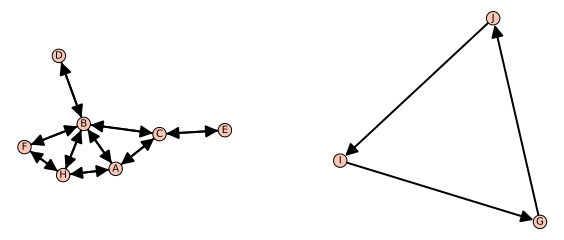
\includegraphics[width=\textwidth]{graph}

\subsection*{b)}

\(R^\infty\) is given by:

\[
\begin{array}{l|c|c|c|c|c|c|c|c|c|c}
   & A & B & C & D & E & F & G & H & I & J \\
\hline
A & 1 & 1 & 1 & 1 & 1 & 1 & 0 & 1 & 0 & 0 \\
\hline
B & 1 & 1 & 1 & 1 & 1 & 1 & 0 & 1 & 0 & 0 \\
\hline
C & 1 & 1 & 1 & 1 & 1 & 1 & 0 & 1 & 0 & 0 \\
\hline
D & 1 & 1 & 1 & 1 & 1 & 1 & 0 & 1 & 0 & 0 \\
\hline
E & 1 & 1 & 1 & 1 & 1 & 1 & 0 & 1 & 0 & 0 \\
\hline
F & 1 & 1 & 1 & 1 & 1 & 1 & 0 & 1 & 0 & 0 \\
\hline
G & 0 & 0 & 0 & 0 & 0 & 0 & 1 & 0 & 1 & 1 \\
\hline
H & 1 & 1 & 1 & 1 & 1 & 1 & 0 & 1 & 0 & 0 \\
\hline
I & 0 & 0 & 0 & 0 & 0 & 0 & 1 & 0 & 1 & 1 \\
\hline
J & 0 & 0 & 0 & 0 & 0 & 0 & 1 & 0 & 1 & 1
\end{array}
\]

\subsection*{c)}

As can be seen in the matrix in b), \(R^\infty\) is already reflexive and so the reflexive closure of \(R^\infty\) is the same as \(R^\infty\).

We can easily read of from the matrix that \(R^\infty\) relates all elements in the set \(\{A, B, C, D, E, F, H\}\), that it relates all elements in the set \(\{G, I, J\}\), and that it relates no other elements. From this it's easy to see that \(R^\infty\) is an equivalence relation.

\end{document}